The last trick for our bag to embark on the KFAC journey is linearization.
It is a useful tool whenever we encounter a composition of functions that we would like to convexify.

Consider for example the function $f = g \circ h$ with $f,g,h: \sR \to \sR$ for simplicity.
We know that convexity is preserved under function composition, so if both $g$ and $h$ are convex, then $f$ will be convex.
But what if only one of the two composites is convex, lets say $g$, but $h$ is not?
Well, then we can replace $h$ with an approximation $h'$ that is convex and approximates the original function somewhat well.
Let's say we are interested in only a neighbourhood around $\vx_0$.
Then, we can obtain a simple, convexified approximation $f' \approx f$ in that neighbourhood by linearizing $h$ around $\vx_0$, resulting in a function $(\lin_{\vx_0}(h))(\vx)$.
This involves a first-order Taylor approximation:

\switchcolumn[1]*
\codeblock{linearization}
\switchcolumn[0]

\begin{definition}[Linearization (vector case, \Cref{linearization})]\label{def:vector_linearization}
  Consider a vector-to-vector function $f$ from \Cref{setup:vector_to_vector_function}.
  The linearization of $f$ at an anchor point $\va_0 \in \sR^A$ denoted by $\lin_{\va_0}(f): \sR^A \to \sR^B$ is its first-order Taylor expansion,
  \begin{align*}
    (\lin_{\va_0}(f))(\va) = f(\va_0) + \jac_{\va_0}f(\va_0) (\va - \va_0)\,,
  \end{align*}
  with the Jacobian from \Cref{def:vector_jacobian}.
  Note that $\lin_{\va_0}(f)$ is linear in $\va$ and coincides with the original function at the anchor point, $(\lin_{\va_0}(f))(\va_0) = f(\va_0)$ (also the Jacobian does).
\end{definition}

\begin{definition}[Linearization (tensor case, \Cref{linearization})]\label{def:tensor_linearization}
  The linearization of a tensor-to-tensor function from \Cref{setup:jacobians} at an anchor point $\tA_0 \in \sR^{A_1 \times \ldots \times A_N}$, denoted by $\lin_{\tA_0}(f)$ is defined per-entry as
  \begin{align*}
    \left[
    (\lin_{\tA_0}(f))(\tA)
    \right]_{j_1, \ldots, j_M}
    = f(\tA_0)
    \\
    +
    \sum_{i_1, \ldots, i_N}
    \left[
    \jac_{\tA_0}f(\tA_0)
    \right]_{j_1, \ldots, j_M, i_1, \ldots, i_N}
    \\
    \left[
    \tA - \tA_0
    \right]_{i_1, \ldots, i_N}\,,
  \end{align*}
  with the Jacobian from \Cref{def:general_jacobian}. Note that this is nothing else but the function evaluated at the anchor point plus the JVP (\Cref{def:jvp}) with the distance to the anchor.
\end{definition}

In deep learning, we will often face the situation where $f = g \circ h, \tA \mapsto b = f(\tA)$ and $h$ is non-convex while $g$ is convex.
This means the Hessian of $f$ can be indefinite; but for algorithms we require a positive definite approximation to the Hessian.
We can obtain that by considering the partially linearized function $f' = g \circ \lin_{\tA_0}(h)$, whose Hessian is positive semi-definite. The Hessian of this partially linearized function is called the generalized Gauss-newton (GGN) matrix.

Let's stick to our one-dimensional example for a moment, i.e.\,let $f(x) = (g \circ h)(x) \in \sR$. If we use the chain rule twice, we obtain the following expression for the Hessian:
\begin{align*}
  \hess_x (g \circ h)(x) =
  \jac_x h(x) \cdot \hess_{h(x)} g(h(x)) \cdot \jac_x h(x)
  \\
  +
  \hess_x h(x) \cdot \jac_{h(x)} g(h(x))\,.
\end{align*}
Now, if we take the hessian of the partially linearized function $f'(x) = (g \circ \lin_{x_0}(h))(x)$, and using the shorthand $h' = \lin_{x_0}(h)$ the second term disappears as the linear function's Hessian is zero:
\begin{align*}
  \hess_x (g \circ h')(x) =
  \jac_x h'(x) \cdot \hess_{h'(x)} g(h'(x)) \cdot \jac_x h'(x)
  \\
  +
  \underbrace{\hess_x h'(x)}_{= 0} \cdot \jac_{h'(x)} g(h'(x))\,.
\end{align*}
If we evaluate both equations at the anchor point, setting $x = x_0$, we obtain that the first terms coincide.

\begin{figure}[!h]
  \centering
  \begin{tikzpicture}[%
    font=\scriptsize,%
    thick,
    box/.style = {rectangle, draw=black, rounded corners, fill=VectorGray!50},%%
    ]
    \node[box] (A) at (0,0) {$f = g \circ h: \tA \mapsto \tB \mapsto c$};
    \node[box] (B) at (4,0) {$\tH_{\tA}c$};
    \node[box, align=center] (C) at (0,-2.5) {%
      $\tilde{f}_{\tA_0} = g \circ \lin_{\tA_0} h$\\%
    };
    \node[box, align=center] (D) at (4,-2.5) {%
      $\tG_{\tA}f(\tA)$
      \\
      $=$\\%
      $\tH_{\tA} f'_{\tA_0}(\tA)|_{\tA_0 = \tA}$\\%
    };
    \draw[-Stealth] (A.east) -- node[fill=white] {$\tH$} (B.west);
    \draw[-Stealth] (A.south) -- node[fill=white, align=center] {partially linearize $f$ \\
      around some $\tA_0$} (C.north);
    \draw[-Stealth] (C.east) -- node[fill=white, align=center] {$\tH$, then\\ set\\ $\tA_0 = \tA$} (D.west);
    \draw[-Stealth] (B.south) -- node[fill=white] {matricize $\tH_{\tA}b$} (D.north);
  \end{tikzpicture}
  \caption{Taking the Hessian and partially linearization commute and lead to the same GGN. All operations also commute with flattening the function versus matrizicing the Hessian tensor, so we can apply any flattening scheme on top to obtain the $\rvec$- and $\cvec$-GGN matrices matrices.}
\end{figure}

We will not use the linearization aspect explicitly in the computation, but instead rely on GGN-vector products which can be built from the previously introduced autodiff operations.
We first provide the definition of the GGN in the matrix and tensor case, before we show how to compute the GGN-vector product.

\switchcolumn[1]*
\codeblock{ggns}
\switchcolumn[0]

\begin{setup}[Composite vector-to-vector-to-scalar function]\label{setup:composite_vector_to_vector_to_scalar_function}
  Let
  \begin{align*}
    f: \sR^{A} &\to \sR
    \\
    \va &\mapsto c = f(\va)
  \end{align*}
  be the composite of a vector-to-vector function $h$ and a vector-to-scalar function $g$, that is
  \begin{align*}
    f = g \circ h: \sR^A &\to \sR^B \to \sR
    \\
    \va &\mapsto \vb = h(\va) \mapsto c = g(\vb)\,.
  \end{align*}
\end{setup}

\begin{definition}[Generalized Gauss-Newton (GGN) matrix (vector case)]\label{def:vector_ggn}
  The GGN matrix of a vector-to-vector-to-scalar function $f$ from \Cref{setup:composite_vector_to_vector_to_scalar_function}, $\ggn_{\va} f(\va) \in \sR^{A \times A}$ is
  \begin{align*}
    \ggn_{\va} f(\va)
    =
    (\jac_{\va} \vb)^{\top}
    (\hess_{\vb} c)
    (\jac_{\va} \vb)\,,
  \end{align*}
  i.e.\,the second composite's Hessian, left- and right-multiplied with the first composite's Jacobian.
\end{definition}

\switchcolumn[1]*
\codeblock{ggn_rosenbrock}
\switchcolumn[0]

\begin{example}[GGN for the Rosenbrock function, \Cref{ggn_rosenbrock}]
  Consider the 2d Rosenbrock function $f_{\alpha}: \sR^2 \to \sR$ with
  \begin{align*}
    f_{\alpha}(\vx)
    =
    (1 - x_1)^2 + \alpha (x_2 - x_1^2)^2\,.
  \end{align*}
  with some $\alpha > 0$.
  We can express $f_{\alpha} = \ell \circ g_{\alpha}$,\footnote{\url{https://www.brnt.eu/phd/node10.html}}
  \begin{align*}
    g_{\alpha}(\vx) = \begin{pmatrix}
                        x_1 \\
                        \sqrt{\alpha} (x_2 - x_1^2)
                      \end{pmatrix}
    \shortintertext{and convex}
    \ell(\vg) = \vg^\top \vg\,,
  \end{align*}
  namely square loss.

  Linearizing $g_{\alpha}$ w.r.t. $\vx$ around $\vx'$ gives
  \begin{align*}
    g^{\text{lin}}_{\alpha}(\vx) = g_{\alpha}(\vx') + (\jac_{\vx'}g_{\alpha}(\vx')) (\vx - \vx')\,.
  \end{align*}
  with
  \begin{align*}
    \jac_{\vx}g_{\alpha}(\vx)
    =
    \begin{pmatrix}
      1 & 0 \\
      -2 \sqrt{\alpha} x_1 & \sqrt{\alpha}
    \end{pmatrix}\,.
  \end{align*}
  The first way to form the Hessian is to take the Hessian of $f_{\alpha}' = \ell \circ g_{\alpha}^{\text{lin}}$, and evaluate it at $\vx' = \vx$,
  \begin{align*}
    (\hess_{\vx} f_{\alpha}'(\vx))|_{x=x'}
    \\
    =
    2 (\jac_{\vx} g_{\alpha}(\vx))|_{x=x'}^{\top}
    (\jac_{\vx} g_{\alpha}(\vx))|_{x=x'}
    \\
    =
    2
    \begin{pmatrix}
      1 + 4\alpha x_1^2& -2 \sqrt{\alpha} x_1\\
      -2 \sqrt{\alpha} x_1 & \alpha
    \end{pmatrix}
  \end{align*}
  This matrix is PSD because it is an outer product of two matrices.
  It is also different from the Hessian matrix
  \begin{align*}
    \hess_{\vx} f_{\alpha}(\vx)
    =
    \begin{pmatrix}
      2 + 12 \alpha x_1^2 - 4 \alpha x_2 & -4 \alpha x_1 \\
      -4 \alpha x_1 & 2 \alpha
    \end{pmatrix}
  \end{align*}
  \begin{figure}[H]
    \centering
    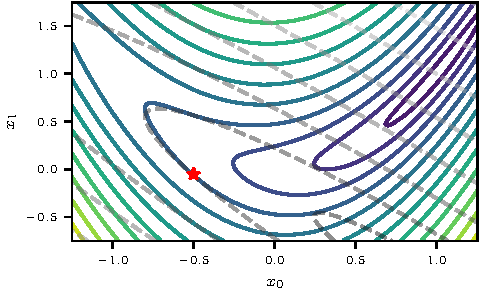
\includegraphics[width=\linewidth]{../kfs/plots/linearized_rosenbrock.pdf}
    \caption{The 2d Rosenbrock function $f_{\alpha=10}$ (solid contour lines) with and its approximation $f'_{\alpha=10, \vx'} = \ell \circ g^{\text{lin}}_{\alpha=10, \vx'}$ (dashed contour lines) when partially linearizing it around an anchor $\vx'$ (star).}
  \end{figure}
\end{example}

\begin{setup}[Composite tensor-to-tensor-to-scalar function]\label{setup:composite_tensor_to_tensor_to_scalar_function}
  Let the tensor-to-scalar function
  \begin{align*}
    f: \sR^{A_1 \times \ldots \times A_N} &\to \sR
    \\
    \tA &\mapsto c = f(\tA)
  \end{align*}
  be the composite of a tensor-to-tensor function $h$ and a tensor-to-scalar function $g$, that is
  \begin{align*}
    f = g \circ h: &\sR^{A_1 \times \ldots \times A_N} \to \sR^{B_1 \times \ldots \times B_M}  \to \sR
    \\
                   &\tA \mapsto \tB = h(\tA) \mapsto c = g(\tB)\,.
  \end{align*}
\end{setup}

\begin{definition}[Generalized Gauss-Newton (GGN) tensor (\Cref{ggns})]\label{def:general_ggn}%
  The GGN tensor of a tensor-to-tensor-to-scalar function $f$ from \Cref{setup:composite_tensor_to_tensor_to_scalar_function}, $\ggn_{\tA} f(\tA) \in \sR^{A_1 \times \ldots \times A_N \times A_1 \times \ldots \times A_N}$ is the Hessian of the partially linearized function $f' = g \circ \lin_{\tA_0}(h)$, evaluated at the anchor point $\tA_0 = \tA$.
  \begin{align*}
    \tG_{\tA} f(\tA)
    =
    \hess_{\tA} \tilde{f}(\tA)|_{\tA_0 = \tA}\,.
  \end{align*}
  where $\tilde{f} = g \circ \lin_{\tA_0}(h)$.

  We can express this tensor as a tensor contraction between the Jacobians and Hessians of the two composites, i.e.\,
  \begin{align*}
    [\tG_{\tA} f(\tA)]_{i_1, \ldots, i_N, j_1, \ldots, j_N}
    \\
    =
    \textcolor{VectorPink}{\sum_{k_1, \dots, k_M}}
    \textcolor{VectorBlue}{\sum_{l_1, \dots, l_M}}
    & [\jac_{\tA} \tB]_{\textcolor{VectorPink}{k_1, \dots, k_M}, i_1, \dots, i_N}
    \\
    &[\hess_{\tB} c]_{\textcolor{VectorPink}{k_{1}, \ldots, k_{M}}, \textcolor{VectorBlue}{l_{1}, \ldots, l_{M}}}
    \\
    &[\jac_{\tA} \tB]_{\textcolor{VectorBlue}{l_1, \ldots, l_M}, j_1, \ldots, j_N}\,.
  \end{align*}
\end{definition}
This expression seems daunting at first, so we will convert things back to matrix notation very soon. Before doing that, let's introduce multiplication with the GGN:

\switchcolumn[1]*
\codeblock{ggn_product}
\switchcolumn[0]

\begin{definition}[GGN-vector-product (GGNVP, \Cref{ggn_product})]\label{def:ggnvp}%
  Consider the GGN tensor of a tensor-to-tensor-to-scalar function $f$ from \Cref{setup:composite_tensor_to_tensor_to_scalar_function,def:general_ggn}.
  The GGN-vector-product (GGNVP) $\tU \in \sR^{A_1 \times \ldots \times A_N}$ with a tensor $\tV \in \sR^{A_1 \times \ldots \times A_N}$ from the input domain is
  \begin{align*}
    &[\tU]_{i_1, \dots, i_N}
    \\
    &=
      \sum_{j_1, \dots, j_N}
      [\tG_{\tA} f(\tA)]_{i_1, \dots, i_N, j_1, \dots, j_N}
      [\tV]_{j_1, \dots, j_N}\,,
  \end{align*}
  and decomposes into a JVP, HVP, and JVP when applying the composition from \Cref{def:general_ggn}.
\end{definition}
This is easiest to see for the vector-to-vector-to-scalar case where $\tA, \tB, \tU, \tV \to \va, \vb, \vu, \vv$ and $\vu = (\jac_{\va}\vb)^{\top} (\hess_{\vb} c) (\jac_{\va} \vb) \vv$, which can be written as a matrix chain and computed without explicitly building up any of the matrices in memory~\cite{schraudolph2002fast}.

\paragraph{Matricization} As for the Hessian and Jacobian, we can flatten the both composite functions before applying the partial linearization and taking the Hessian to obtain the GGN.
This is equivalent to matricizing the GGN tensor from \Cref{def:general_ggn}.
And it is also equivalent to matricizing the Hessians and Jacobians in the general definition.

\begin{definition}[$\cvec$ and $\rvec$ GGN matrices, \Cref{ggns}]\label{def:vec_ggns}
  For a tensor-to-tensor-to-scalar function $f$ from \Cref{setup:composite_tensor_to_tensor_to_scalar_function}, we define the $\cvec$ and $\rvec$ GGN matrices by flattening the composite functions before applying the partial linearization and taking the Hessian. This yields the flattened GGN matrices $\ggn^{\vec}_{\tA}f(\tA) \in \sR^{A_1 \cdots A_N \times A_1 \cdots A_N}$ where $\vec \in \{\cvec, \rvec\}$ which can be written as matrix chain
  \begin{align*}
    \ggn^{\vec}_{\tA} f(\tA)
    =
    (\jac^{\vec}_{\tA} \tB)^{\top}
    (\hess^{\vec}_{\tB} c)
    (\jac^{\vec}_{\tA} \tB)\,.
  \end{align*}
  using the previously defined flattened Hessians (\Cref{def:cvec_hessian,def:cvec_hessian}) and Jacobians (\Cref{def:cvec_jacobian,def:rvec_jacobian}).
\end{definition}

Again, it is important to emphasize that the matrix GGN depends on the flattening scheme.
To emphasize this point, we conclude this section with the following:

\switchcolumn[1]*
\codeblock{ggns_linear_regression}
\switchcolumn[0]

\begin{example}[GGN of linear regression (\Cref{ggns_linear_regression})]
  Consider the least squares objective
  \begin{align*}
    \gL(\mW) = \sum_n \ell_n(\mW)
  \end{align*}
  where $\ell_n = c_n \circ f_n$ is the composition of a linear classifier and square loss
  on a data point labeled $n$, that is
  $f_n(\mW) = \mW \vx_n$ and $c_n(\vz) = \left\lVert \vz - \vy_n \right\rVert^2_2$.

  Using the shorthands $\vf_n \coloneq f_n(\mW)$ and $c_n \coloneq c_n(\vf_n)$, the matrix GGNs are given by
  \begin{align*}
    \ggn_{\mW}^{\vec}\gL(\mW)
    \coloneq
    \sum_n
    \ggn_{\mW}^{\vec} \ell_n(\mW)
    \\
    =
    \sum_n
    (\jac^{\vec}_{\mW} \vf_n)^{\top}
    (\hess^{\vec}_{\vf_n} c_n)
    (\jac^{\vec}_{\mW} \vf_n)\,.
  \end{align*}
  We can use the results from previous examples, specifically \Cref{jacobians_linear_layer,ex:square_loss_hessian}, to obtain the following expressions
  \begin{align*}
    \ggn_{\mW}^{\cvec}\gL(\mW)
    &=
      \left(
      \sum_n \vx_n \vx_n^{\top}
      \right)
      \otimes \mI
    \\
    \ggn_{\mW}^{\rvec}\gL(\mW)
    &=
      \mI
      \otimes
      \left(
      \sum_n \vx_n \vx_n^{\top}
      \right)
  \end{align*}
\end{example}
Two interesting observations about this result are (i) both GGNs are a Kronecker product (ii) whose order of factors depends on the flattening scheme we are using.
This already hints at using a Kronecker product to approximate the exact GGN, which is what KFAC aims to do.


%%% Local Variables:
%%% mode: latex
%%% TeX-master: "../main"
%%% End:
